\documentclass[]{article}

%opening
\title{{\bf Practical 1}: Predicting the Efficiency of Organic Photovoltaics}
\author{Neil Chainani
		Avery Faller}

\usepackage[OT1]{fontenc}
\usepackage[colorlinks,citecolor=blue,urlcolor=blue]{hyperref}
\usepackage[pdftex]{graphicx}
\usepackage{subfig}
\usepackage{fullpage}
\usepackage{palatino}
\usepackage{mathpazo}
\usepackage{amsmath}
\usepackage{amssymb}
\usepackage{color}
\usepackage{todonotes}
\usepackage{listings}
\usepackage[utf8]{inputenc}
\usepackage[english]{babel}


\renewcommand{\baselinestretch}{1.25	}

\begin{document}
	
\maketitle

\section{Technical Approach}
\subsection*{How did you tackle the problem?}
\begin{figure}[h]
	\centering
	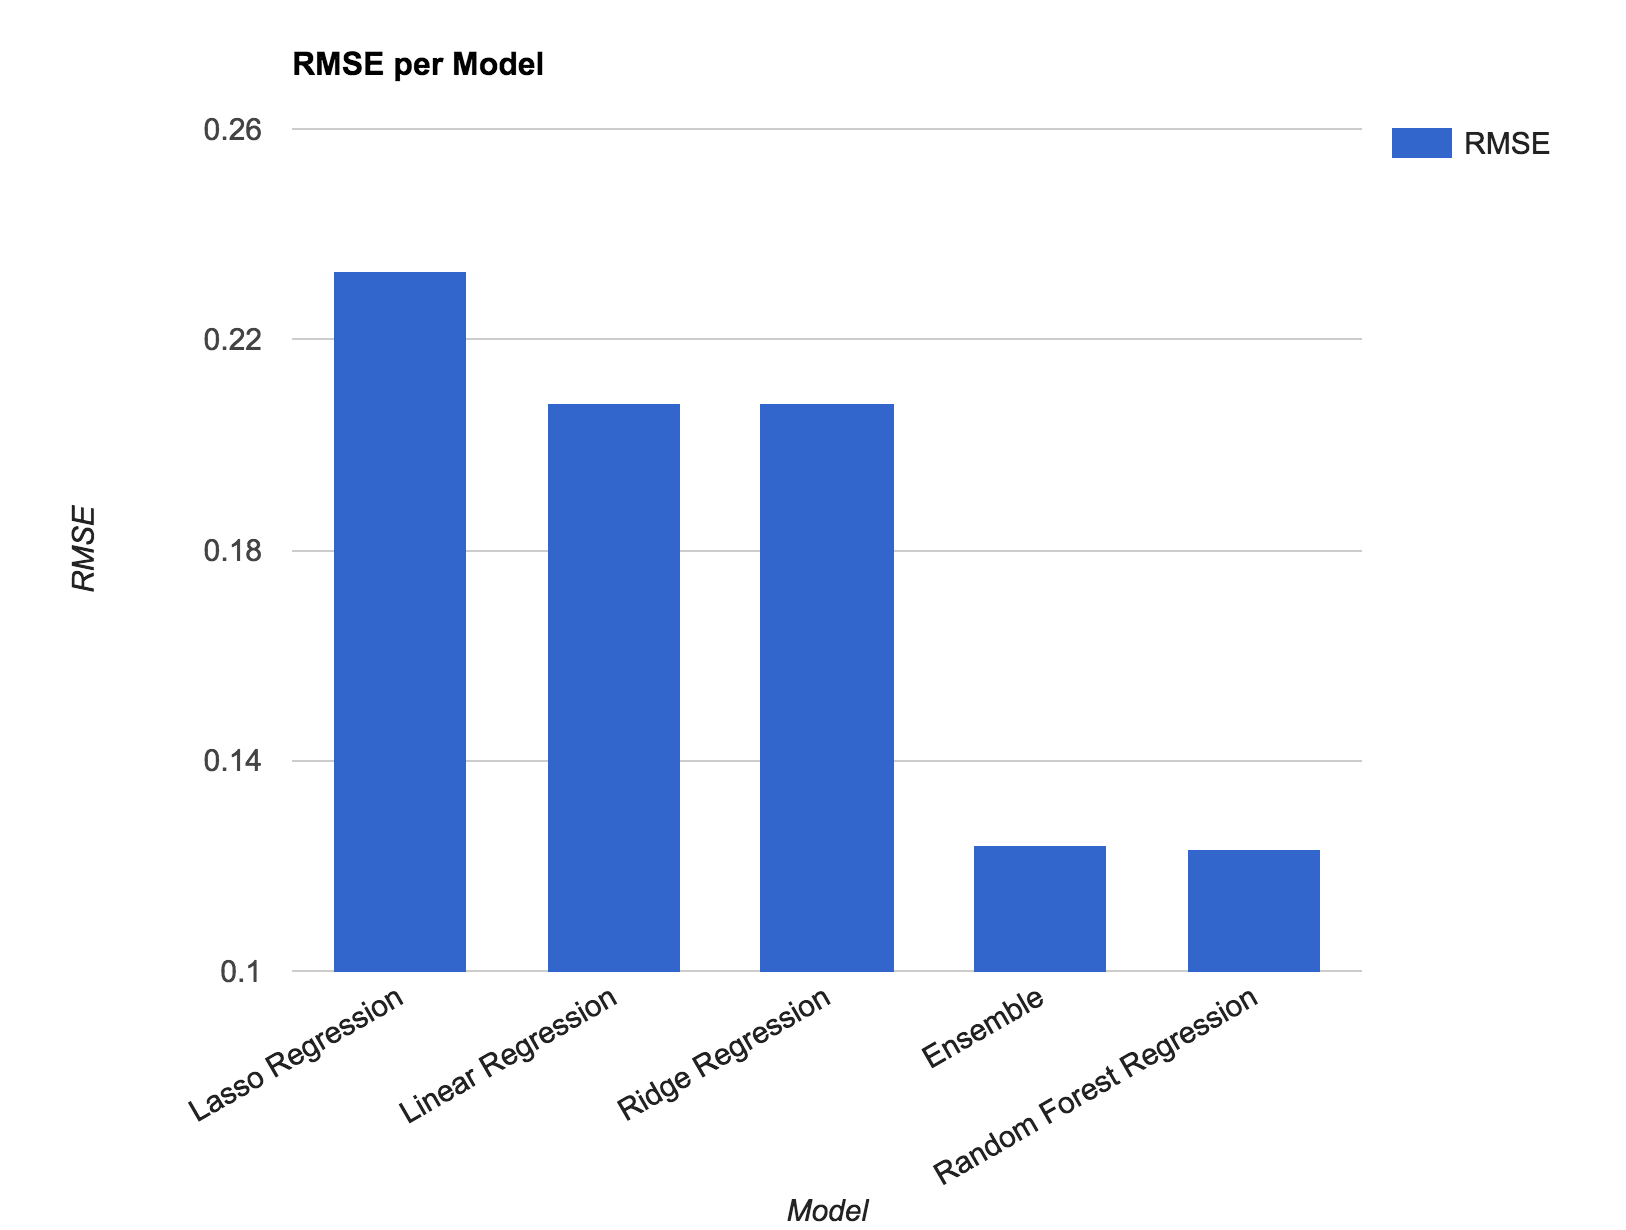
\includegraphics[width=0.7\textwidth]{ModelComparison}
	\caption{Model Comparison}
\end{figure}

\begin{flushleft}
	We began with the supplied Sample IPython notebook, which applied basic linear regression and random forests on the 256 provided binary features. The first step in our approach was to determine the most effective machine learning model. We compared the root mean squared error (RMSE) for a number of unoptimized models, including Linear Regression, Lasso Regression, Ridge Regression, Random Forest Regression and an ensemble of the four, and determined that the Random Forest Regressor had the lowest RMSE. We also tried K-nearest neighbors, and Polynomial Interpolation, but Random Forest Regression was better and faster than both of them.
	\newline\newline
	Once we had established that Random Forest Regressors were the model to go with, we began the process of engineering the most effective features while simultaneously tuning our Random Forest Regressor to produce the best predictions.  We had a hunch that some of the given binary features were not useful, so we summed up each of the columns. We saw immediately that out of the 256 features, 244 of them had a value of 0 for every molecule, so we dropped these columns for the sake of efficiency.
	\newline\newline
	It was clear that the remaining provided binary features were hardly sufficient, so we decided to delve into the SMILES feature. This complex string held a wealth of information regarding the chemical properties of the molecule, however, neither of us have much domain knowledge in chemistry, so for our feature extraction, we mainly treated the SMILES as a text analysis problem.
	\newline\newline
	We first applied a basic set of features on the counts of the characters within the strings. We discovered that there were only 21 distinct case-sensitive characters present in the string, and added an indicator variable for each of these as a feature. 
	\newline\newline
	\begin{figure}[h]
		\centering
		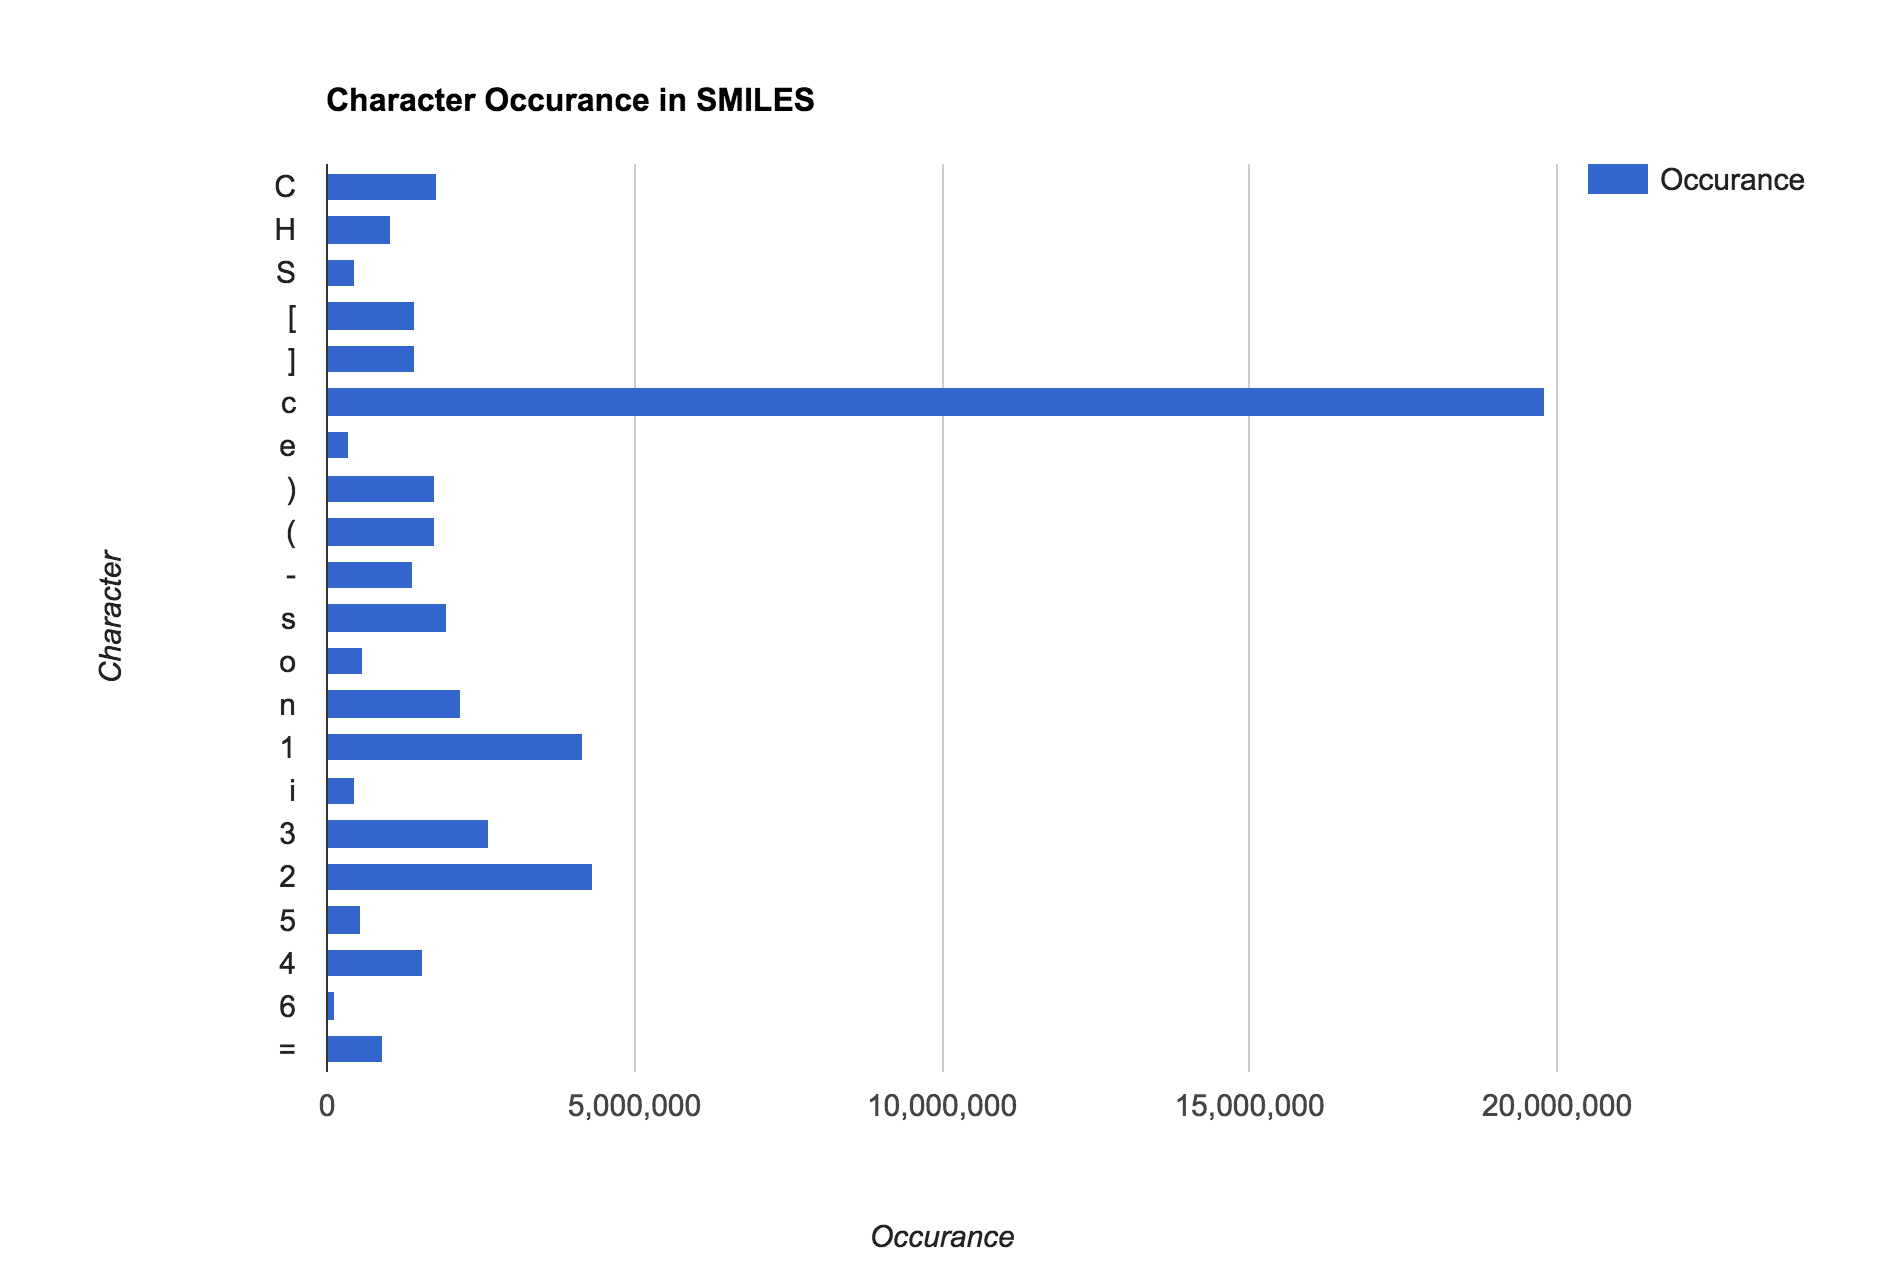
\includegraphics[width=0.8\textwidth]{CharacterOccurance}
		\caption{Occurrences of all 21 characters}
	\end{figure}
	\newline\newline
	We then pursued more deliberate feature engineering using our limited knowledge of chemistry. We extracted features, such as the length of the SMILES string, the percentage of the SMILES string that was uppercase and lowercase (which indicates it is aromatic). We picked out specific molecules, such as ‘o1cccc1’ and ‘n1ccccc1’, and created indicator features for them.  Finally, we looked at whether the SMILES string began or ended with certain molecules. 
	\newline\newline
	The model continued to improve, but we were certain there was more manipulation to be done. Developing features by hand was time consuming, so we auto-generated features for the top N bi-grams (pairs of consecutive characters), and tuned the number N high enough until we saw diminishing returns given time constraints. Because of how much success this reaped, we repeated this process for 3-grams, 4-grams and 5-grams, and were able to bring our RMSE down significantly with each additional set of features.  However, as our RMSE improved, it became increasingly difficult to lower, and the runtime of our Random Forest Regressor increased dramatically.
	\newline\newline
\end{flushleft}
\section{Results}
\subsection*{How well did your set of predictions do?}
\begin{flushleft}
	\begin{figure}[h]
		\centering
		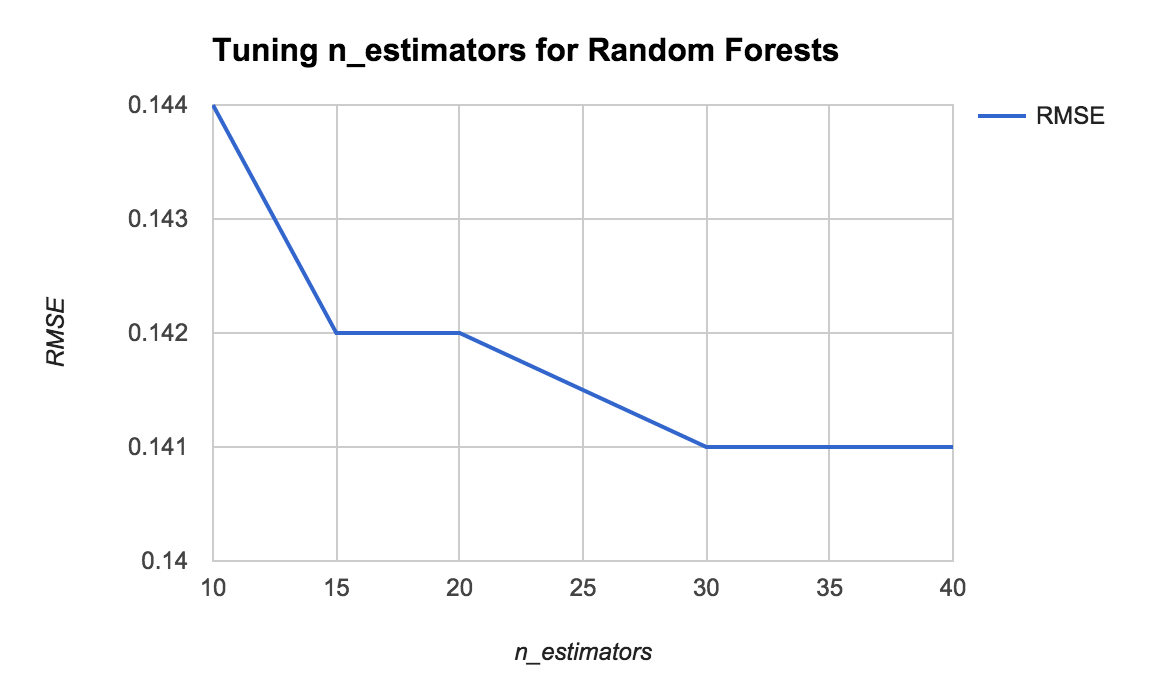
\includegraphics[width=0.8\textwidth]{n_estimators}
		\caption{Tuning number of trees for Random Forests}
	\end{figure}
	We started from the Random Forest baseline given in the sample code.  This code generates predictions with a RMSE of .272.  Our biggest drop in RMSE was our first one.  By simply adding an indicator column for each symbol in the SMILES dictionary and iterating over hyperparameters for the Random Forest Regressor, we dropped our RMSE down to .141.
	\newline\newline
	After performing feature engineering to build up 50 custom features our RMSE dropped again to .1260. After this drop, it became much harder to improve.  We once again turned to tuning our Random Forest Regressor by customizing the min-samples-split parameter which brought us down to .1230.
	\newline\newline
	\begin{figure}[h]
		\centering
		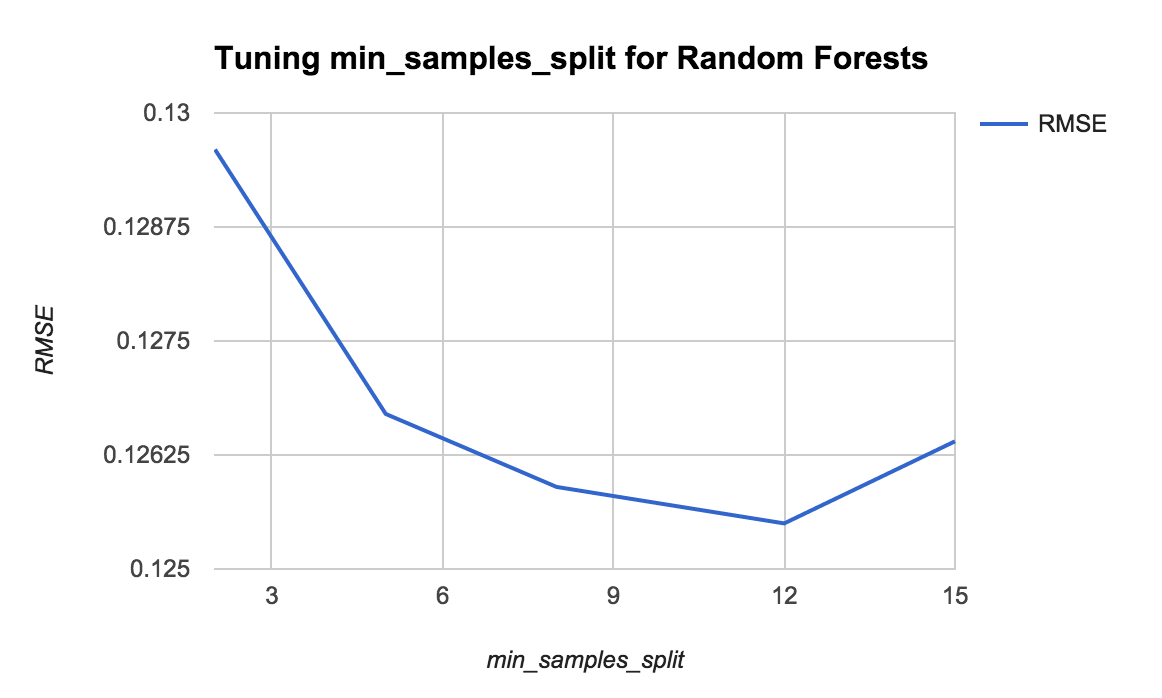
\includegraphics[width=0.8\textwidth]{min_samples_split}
		\caption{Tuning min samples split for Random Forests}
	\end{figure}
	\newline\newline
	Adding Bigrams and tuning how many we used brought us further down to .1011.  By continuing in this vein, adding Trigrams dropped us further to .0864.  Quadgrams brought the RMSE to .0809 and Quintgrams further lowered the RMSE to .0777.
	\newline\newline
	All this is to say that adding additional features continued to lower our RMSE, however these improvements came at the cost of potentially overfitting and significantly increasing our running time.  Fitting the Random Forest could take on the order of two hours with all of our features turned on.
\end{flushleft}
\section{Discussion}
\subsection*{What was your thought process for your approach?}
\begin{flushleft}
	Our work had two major parts to it: selecting the best model, and engineering the best set of features.  Selecting the best model was mainly about testing, but those tests agreed with our thoughts:  Random Forests work best with lots of data, and we had no shortage of data in this Practical.  
	\newline\newline
	Random Forests also have the advantage of being less prone to overfitting.  So, with that fact in mind, we set about building lots of features to fit our model with.  We built around 50 features by hand that looked for specific molecules or other special features of the SMILES strings.  However, this was taking a long time to create features and test them, so we set about finding a way to automate feature creation.  We choose to do this by building N-grams, starting with monograms, and working our way up to quintgrams.  By simply piling lots of features into our dataframe, we were able to hand off our limited understanding of chemistry to the sheer quantity of features we were able to generate.  In the end we had over 600 features.  Although undoubtedly some of these features were quite bad, or even detrimental to the model, by providing enough of them with a sufficient amount of data (which we were given), Random Forest Regression was able to discover which were the most significant predictors.
	\newline\newline
	\begin{figure}[h]
		\centering
		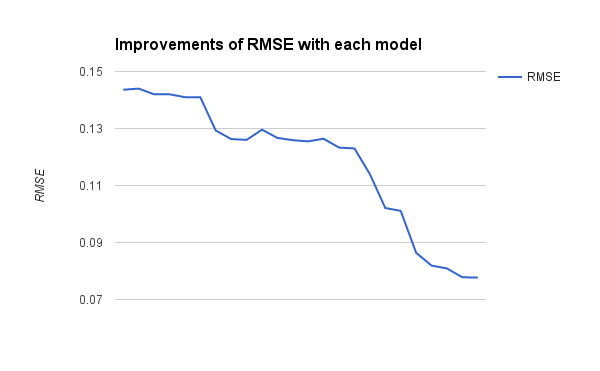
\includegraphics[width=0.8\textwidth]{overall_rmse}
		\caption{Seeing the RMSE fall as the model improves}
	\end{figure}
\end{flushleft}	

\end{document}
